\section{Studies on the \nonprompt photon background}
\label{sec:phFRstudies}
The uncertainty on the fake photon background has different sources,
depending on whether it is estimated with simulation or using a data-driven method:
\begin{enumerate}
\item the uncertainty on the value of the fake rate itself,
      mainly due to the amount of data in the measurement region $\PZ+\text{L}$;
\item the uncertainty due to the limited number of events
      in the fake rate application region, especially for the four lepton channel;
\item the different background composition between the measurement and application region;
\item the mismodelling of the simulation of the processes that result in \nonprompt photons
      and their identification by the detector and the reconstruction algorithm.
\end{enumerate}

The first three affect only the data-driven estimate,
while the last is the main uncertainty when using the simulation to estimate the fake photon background.
However, it also impacts the data-driven method, as the prompt photons in the measurement region are subtracted
using the simulation of the $\PZ+\PGg$ process.

%% \note{We should decide which uncertainties are included in the (arbitrary) flat 50\usep\% normalization uncertainty, if any.}

%% The first source is the uncertainty on the fake rate itself, which is measured in data in the $\PZ+\text{L}$ region.
%% The second source is the limited amount of data in the fake rate application region.
%% Another source is the difference in background composition between the fake rate measurement region and the signal region.
%% These affect only the data-driven estimate.

%% When using the simulation of the \nonprompt photon background, the main uncertainty
%% is the modelling accuracy of such process in the various background samples.
%% This uncertainty is difficult to evaluate, and the method used in this analysis to estimate it
%% is to compare the fake rate measured in data to the one calculated in the samples with \nonprompt photons.

\subsection[Uncertainty on the normalization of gg to 4l]{Uncertainty on the normalization of $\Pg\Pg \to 4\Pl$}
\label{gg4l_normgroup}
The normalization uncertainty on the three samples $\Pg\Pg \to 4\Pe$, $\Pg\Pg \to 2\Pe2\PGm$ and $\Pg\Pg \to 4\PGm$
can be applied as a single nuisance parameter common to all of them
or as three separate parameters that are determined separately in the fit.

The difference between the two approaches, which is expected to be really small,
is evaulated by comparing the expected significances, as shown in Table \ref{tab:grupnorm_cross_check_significance}.
As anticipated, the changes are negligible, usually less than or equal to $0.1\usep\sigma$,
except for the last strategy, where the expected significance changes by $\approx 0.2\usep\sigma$.

\begin{table}
  \caption{Expected significance with the various strategies,
    when the uncertainty on the normalization of the $\Pg\Pg \to 4\Pl$ samples is
    grouped into a single parameter or split into three, one for each final state.}
  \label{tab:grupnorm_cross_check_significance}
  \centering
  \begin{tabular}{l l l c c}
    \toprule
    \multicolumn{3}{c}{Strategy} & \multirow{2}{*}{\shortstack{Significance\\(single)}} & \multirow{2}{*}{\shortstack{Significance\\(split)}}\\
    \noalign{\vspace{.1ex}}\cline{1-3}\noalign{\vspace{.1ex}}
    Photon ID & \nonprompt \PGg & Variable\\
    \midrule
    Cut-based Loose  & data-driven & $m_{\PZ\PZ\PGg}$ & 4.54 & 4.54 \\
    Cut-based Loose  & simulation  & $m_{\PZ\PZ\PGg}$ & 4.60 & 4.65 \\
    Cut-based Loose  & simulation  & $\pt^\PGg$       & 4.53 & 4.57 \\
    MVA ({\tt wp90}) & simulation  & $m_{\PZ\PZ\PGg}$ & 5.06 & 5.13 \\
    MVA ({\tt wp90}) & simulation  & $\pt^\PGg$       & 5.00 & 5.07 \\
    MVA ({\tt wp80}) & simulation  & $m_{\PZ\PZ\PGg}$ & 5.20 & 5.30 \\
    Kinematic        & simulation  & MVA score        & 5.34 & 5.55 \\
    \bottomrule
  \end{tabular}
\end{table}


\subsection{Uncertainty on the fake rate}
The photon fake rate is also affected by the amount of data in the measurement region.
Its impact is evaluated by propagating this uncertainty
through the per-event transfer factor (see Equation~\ref{eq:fakeRate_explanation_part2}),
and constructing the systematic variations of the histograms used for the fit.
It results in a decrease of the expected significance of $\approx 0.09\usep\sigma$.

\subsection{Number of events in the application region}
A major contribution to the uncertainty of the data-driven estimate of the fake photon background
is the limited amount of data in the application region, especially in the four lepton channel.
It is modelled with a Gamma function (see Equation~\ref{eq:gammadef}).
The application of this uncertainty reduces the expected significance by $\approx 0.02\usep\sigma$
in the inclusive region of the four lepton channel.

\subsection{Unified fake rate for all data-taking periods}
As stated in Section~\ref{sec:fake_photons_background}, the photon fake rate is derived separately for the four data-taking periods of \Run2.
The alternative approach is to derive a single fake rate with a smaller statistical uncertainty,
at the cost of increasing the correlation between the different periods.
The resulting fake rate is shown in Figure~\ref{fig:phFR_Run2}.

The effect is expected to be small due to the limited impact of the uncertainty on the fake rate,
which is purely due to the amount of data in the measurement region.
Indeed, using an unique fake rate correlated among the data-taking periods
results in an increase of the expected significance with the data-driven approach
of $\approx 0.036\usep\sigma$.

\begin{figure}
  \centering
  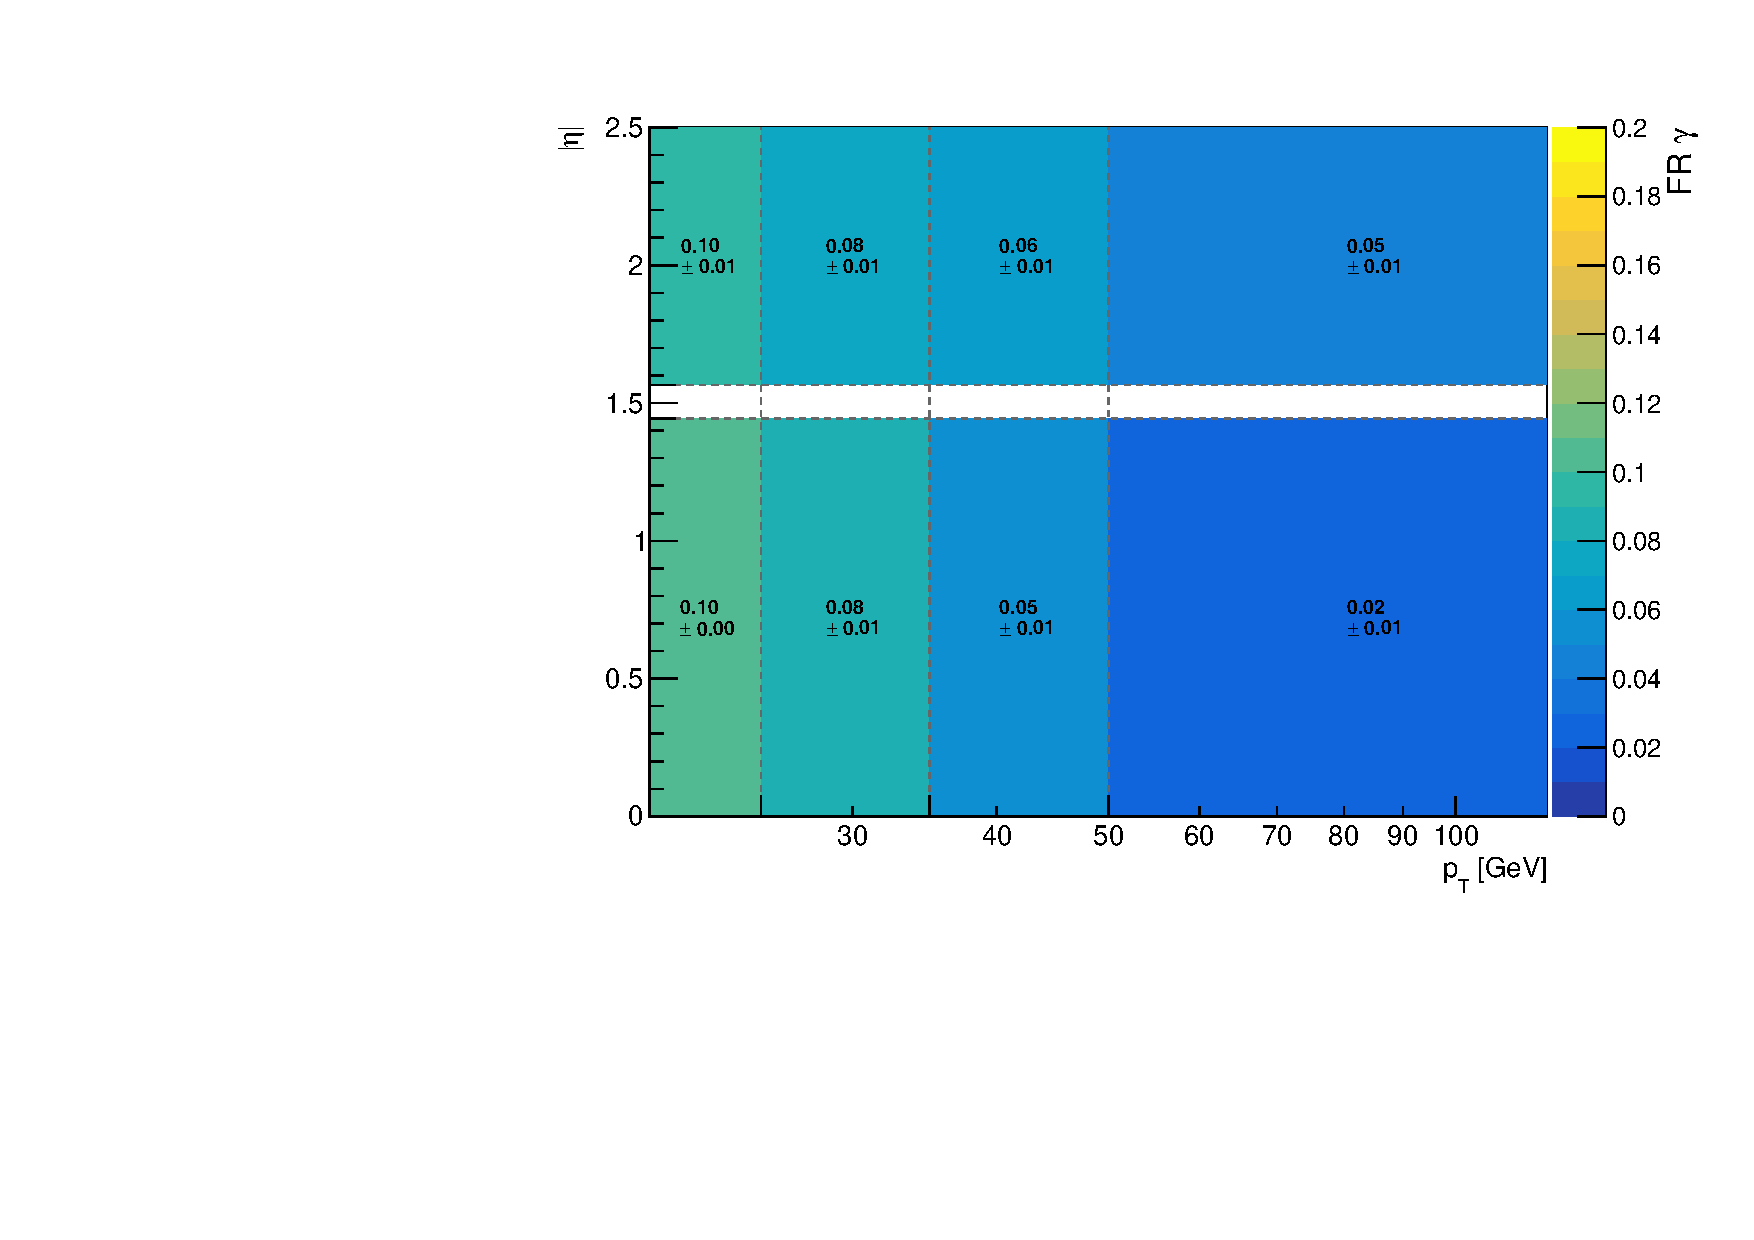
\includegraphics[height=.333333\textheight]{Figures/PhFR/FR_VLtoL_pt-aeta_data-ZGToLLG_Run2.pdf}
  \caption{Photon fake rate measured in the $\PZ+\rm{L}$ region combining events from the four data-taking periods of \Run2.}
  \label{fig:phFR_Run2}
\end{figure}

%% \note{This is the comparison between ``uniqueFR'' and ``ARstat-restorePhFR-groupnorm''.
%% Looking at [control-uniqFR], which is derived using a single FR while leaving the datacard entries \textbf{uncorrelated},
%% suggests that the reduction in the FR uncertainty results in ${+}0.041\usep\sigma$,
%% while the correlation between channels reduces the significance by ${-}0.005\usep\sigma$.}

%% phsigdef                               4.53923  result presented in v1.0
%% restorePhFR-groupnorm-phsigdef         4.45033  (re-)added uncertainty on measured PhFR, stat from CRLFR
%% ARstat-restorePhFR-groupnorm-phsigdef  4.43012  Added gmN representing the stat in the AR (CR4P_1F), uncorrelated between years
%% control-uniqFR                         4.47124  Run with a single FR, derived grouping all events in CRLFR for Run2; do not change the datacard
%% uniqFR                                 4.46641  Make the PhFR correlated, since we used the same values in all the years
